\section{SURF}
SURF (Speeded Up Robust Features) is a local feature transform algorithm proposed by Herbert Bay, Tinne Tuytelaars, and Luc Van Gool in 2006\cite{Bay2006}. Compared to SIFT\cite{Lowe1999}, the authors claim the SURF detector and descriptor, to be faster and more robusit against various image transformations.

\subsection{Keypoint Detection}
The SURF keypoint detection is based on determinant of the Hessian matrix. Let us consider an input image $I_{img}(x,y)$ and the scale space representation of the image
\begin{equation}
    L(x, y,\sigma) =  G(x,y,\sigma)*I_{img}(x,y),
\end{equation}
where $G(x,y,\sigma)$ is the Gaussian kernel described in \eqref{eq:Gaussian_kernel}.

The Hessian matrix at scale $\sigma$ is defined as
\begin{equation}
    \mathcal{H}(x, y, \sigma) =
    \begin{bmatrix}
        L_{xx}(x, y, \sigma) & L_{xy}(x, y, \sigma)\\
        L_{xy}(x, y, \sigma) & L_{yy}(x, y, \sigma)
    \end{bmatrix}
\end{equation}
where $L_{xx}(x, y, \sigma)$, $L_{xy}(x, y, \sigma)$ and $L_{yy}(x, y, \sigma)$ are the second order derivatives of the scale space representation of the image at a point $(x, y)$.

As the property of Gaussian filter, that no new structures can appear while going to a lower resolution has been shown not to apply in 2D case \cite{Koenderink1984}, the SURF authors choose to approximate the second order derivatives of Gaussian filter with box filters (shown in \figref{fig:Gauss_box_y}). These allow for the use of integral images, which reduce the computational complexity.

\begin{figure}
    \centering
    \begin{subfigure}{0.24\textwidth}
        \centering
        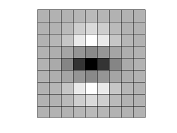
\includegraphics[width=\textwidth]{Figures/surf/y_gauss.png}
        \label{fig:y_gauss}
    \end{subfigure}
    \begin{subfigure}{0.24\textwidth}
        \centering
        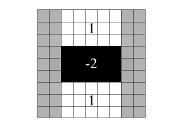
\includegraphics[width=\textwidth]{Figures/surf/y_box.png}
        \label{fig:y_box}
    \end{subfigure}
    \caption[Gaussian second order derivative in the $y$-direction and its approximation using box filters]{Gaussian second order derivative in the $y$-direction and its approximation using box filters \cite{Bay2006}}

    \label{fig:Gauss_box_y}
\end{figure}

Let us denote the approximations by $D_{xx}$, $D_{xy}$, and $D_{yy}$. The relative weights in the calculation of determinant of Hessian need to be weighted with by $0.9$, which yields
\begin{equation}
    \text{det}(\mathcal{H}) = D_{xx} * D_{yy} - (0.9 * D_{xy})^{2}.
\end{equation}

Due to the use of box filters and integral images, any size of the box filter can be applied to the original image at the same speed directly. Therefore, the scale space is created by the use of up-scaled filters of size $9\times9$, $15\times15$, $21\times21$, $27\times27$, etc. For each octave, the difference between filter sizes is doubled (from $6$ to $12$ to $24$).

As the box filter layout remains the same, the corresponding Gaussian filter scales accordingle. The $9\times9$ box filter corresponds to a Gaussian filter with the scale $\sigma = 1.2$. From this, we can calculate the corresponding Gaussian filter scale for each box filter size.

To select the keypoints, non-maximum suppression in the $3\times3\times3$ neighbourhood of each point is applied. The maxima of the determinant of the Hessian matrix are then interpolated the same way as in the SIFT algorithm (using quadratic Taylor expansion).

\subsection{Keypoint Description}
First, we need to ensure descriptor's invariance to rotation. For the keypoint, we calculate the Haar-wavelet responses in $x$ and $y$ direction in a circular neighbourhood of $6s$, where $s$ is the Gaussian filter scale at which the keypoint was found. Integral images are used for speeding up the process.

The wavelet responses are then weighted with a Gaussian($\sigma = 2.5 s$) centered at the keypoint. The weighted responses are represented as vectors in a space with the $x$ response being a vector along the $x$ axis, and the $y$ response being a vector along the $y$ axis. All the vectors within a sliding window of $\frac{\pi}{3}$ are summed, and the longest of the vector is selected as the keypoint orientation.

The descriptor is constructed from a square window the size of $20s$ around a keypoint. The window is then rotated along the keypoint orientation. This window is then divided into $16$ ($4\times4$) square sub-windows. In each sub-window, the features are calculated using $5\times5$ regulary spaced sample points. For these, we calculate the Haar wavelet responses in horizontal and vertical direction, where \say{horizontal} and \say{vertical} are defined in relation to the keypoint orientation. The responses are weighted with a Gaussian($\sigma = 3.3s$), centered at the keypoint.

Let us call the horizontal responses $d_x$ and the vertical responses $d_y$. Over each sub-window, we denote the sum of the responses $\sum d_x$ and $\sum d_y$, and the sum of absolute values of the responses $\sum |d_x|$ and $\sum |d_y|$. The behaviour of these values for different image patterns can be seen in \figref{fig:surf_descriptor}. Combining $\sum d_x$, $\sum d_y$, $\sum |d_x|$, and $\sum |d_y|$ for the each of the $16$ sub-window into a vector, we get a descriptor of length $64$.

\begin{figure}
    \centering
    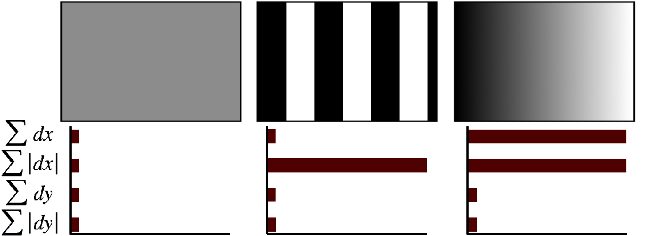
\includegraphics[width=0.8\textwidth]{Figures/surf/surf_descriptor.png}
    \caption[Behaviour of SURF descriptor for different image patterns]{Behaviour of SURF descriptor for different image patterns\cite{Bay2006}}
    \label{fig:surf_descriptor}
\end{figure}
